%%Do not change font size
\documentclass[12pt]{article}
\usepackage{amsthm,amssymb,fullpage}
\usepackage[ruled,vlined,english]{algorithm2e}

\pdfoutput=1
\usepackage{mathpazo}
\usepackage{color}
\usepackage{placeins}
%\usepackage{etoolbox}
%\newbool{submit}
%\setbool{submit}{true}
%\newbool{havealerts}
%\newbool{fullversion}
%\setbool{fullversion}{true}


%\newcommand{\defeq}{\stackrel{\textup{def}}{=}}
%\newcommand{\nfrac}{\nicefrac}
\newcommand{\avg}{{\ensuremath{\mathsf{avg}}\xspace}}
\renewcommand{\epsilon}{\varepsilon}


\usepackage{nicefrac}
\newcommand{\flatfrac}[2]{#1/#2}
\newcommand{\ffrac}{\flatfrac}
\newcommand{\nfrac}{\nicefrac}


\usepackage[compact]{titlesec}
\usepackage{mdwlist}
\usepackage{mathrsfs}
\usepackage{hyperref, geometry, tabularx,graphicx}
\usepackage{amsmath, amsthm, amssymb, enumerate}
\usepackage{fullpage}
\usepackage{latexsym}
\usepackage[capitalize]{cleveref}

\usepackage{tikz}
\usetikzlibrary{decorations.pathreplacing}


%Macros
\newtheorem{lemma}{Lemma}
\newtheorem{theorem}[lemma]{Theorem}
\newtheorem{informaltheorem}[lemma]{Informal Theorem}
\newtheorem{informallemma}[lemma]{Informal Lemma}
\newtheorem{corollary}[lemma]{Corollary}
\newtheorem{definition}[lemma]{Definition}
\newtheorem{proposition}[lemma]{Proposition}
\newtheorem{question}{Question}
\newtheorem{example}[lemma]{Example}
\newtheorem{remark}[lemma]{Remark}
\newtheorem{claim}{Claim}
\newtheorem{fact}{Fact}
\newtheorem{challenge}{Challenge}
\newtheorem{observation}{Observation}
\newtheorem{openproblem}{Open Problem}
\newtheorem{openquestion}{Open question}
\newtheorem{homework}{Homework}
\newtheorem{notation}{Notation}
\newcommand{\todo}[1]{\noindent \colorbox{green}{\begin{minipage}{\linewidth}{\bf TODO:} #1\end{minipage}}}

\newcommand{\beq}{\begin{equation}}
\newcommand{\eeq}{\end{equation}}
%\newcommand{\beas}{\begin{eqnarray*}}
%\newcommand{\eeas}{\end{eqnarray*}}
%
%\newcommand{\poly}{\mathrm{poly}}
%\newcommand{\eps}{\epsilon}
\newcommand{\e}{\epsilon}
%\newcommand{\polylog}{\mathrm{polylog}}
%\newcommand{\rob}[1]{\left( #1 \right)} %Round Brackets
%\newcommand{\sqb}[1]{\left[ #1 \right]} %square Brackets
%\newcommand{\cub}[1]{\left\{ #1 \right\} } %curly brackets
%\newcommand{\rb}[1]{\left( #1 \right)} %Round
%\newcommand{\abs}[1]{\left| #1 \right|} %| |
%\newcommand{\zo}{\{0, 1\}}
%\newcommand{\zonzo}{\zo^n \to \zo}
%\newcommand{\zokzo}{\zo^k \to \zo}
%\newcommand{\zot}{\{0,1,2\}}
\newcommand{\norm}[1]{\left\lVert#1\right\rVert}
%
%\newcommand{\en}[1]{\marginpar{\textbf{#1}}}
%\newcommand{\efn}[1]{\footnote{\textbf{#1}}}
\newcommand{\bR}{\mathbb{R}}

%End macros

\newcommand{\defeq}{\stackrel{{\rm def}}{=}}


%% FROM MARC MACRO FILE


\newcommand{\EE}{\mathbb{E}}
\newcommand{\CC}{\mathbb{C}}
\newcommand{\GG}{\mathbb{G}}
\newcommand{\KK}{\mathbb{K}}
\newcommand{\NN}{\mathbb{N}}
\newcommand{\PP}{\mathbb{P}}
\newcommand{\QQ}{\mathbb{Q}}
\newcommand{\RR}{\mathbb{R}}
\newcommand{\ZZ}{\mathbb{Z}}

\newcommand{\A}{\mathcal{A}}
\newcommand{\B}{\mathcal{B}}
\newcommand{\C}{\mathcal{C}}
\newcommand{\D}{\mathcal{D}}
\newcommand{\E}{\mathcal{E}}
\newcommand{\F}{\mathcal{F}}
\newcommand{\G}{\mathcal{G}}
\renewcommand{\H}{\mathcal{H}}
\newcommand{\I}{\mathcal{I}}
\newcommand{\K}{\mathcal{K}}
\renewcommand{\L}{\mathcal{L}}
\newcommand{\M}{\mathcal{M}}
\newcommand{\N}{\mathcal{N}}
\newcommand{\R}{\mathcal{R}}
\renewcommand{\S}{\mathcal{S}}
\newcommand{\T}{\mathcal{T}}
\newcommand{\U}{\mathcal{U}}
\newcommand{\V}{\mathcal{V}}
\newcommand{\W}{\mathcal{W}}
\newcommand{\X}{\mathcal{X}}
\newcommand{\Y}{\mathcal{Y}}

\newcommand{\bA}{\mathbf{A}}
\newcommand{\bE}{\mathbf{E}}
\newcommand{\bF}{\mathbf{F}}
\newcommand{\bG}{\mathbf{G}}
\newcommand{\bN}{\mathbf{N}}
\newcommand{\bU}{\mathbf{U}}
\newcommand{\bX}{\mathbf{X}}

\newcommand{\ens}[1]{\left\{ #1 \right\}}
\newcommand{\set}[1]{\left\{ #1 \right\}}
\renewcommand{\leq}{\leqslant}
\renewcommand{\geq}{\geqslant}
\renewcommand{\le}{\leqslant}
\renewcommand{\ge}{\geqslant}
\newcommand{\cplx}[1]{\mathcal O \left( #1 \right)}
\newcommand{\floor}[1]{\left \lfloor #1 \right \rfloor}
\newcommand{\ceil}[1]{\left\lceil #1 \right\rceil}
\newcommand{\brackets}[1]{\left[ #1 \right]}
\renewcommand{\angle}[1]{\left\langle #1 \right\rangle}
\newcommand{\donne}{\rightarrow}
\newcommand{\gives}{\rightarrow}
\newcommand{\dans}{\to}
\newcommand{\booleen}{\set{0,1}^*}
\newcommand{\eps}{\varepsilon}
\renewcommand{\implies}{~\Rightarrow~}
\newcommand{\tildarrow}{\rightsquigarrow}
\newcommand{\blank}{\texttt{\char32}}
\newcommand{\trans}[1]{\xrightarrow{#1}}
\newcommand{\rules}[1]{\xrightarrow{#1}}
\newcommand{\wtf}[1]{\Huge\textcolor{red}{WTF ?! #1}\normalsize}
\newcommand{\argmin}{\text{argmin}}
\newcommand{\rainbowdash}{\vdash}
\newcommand{\notrainbowdash}{\nvdash}
\newcommand{\rainbowDash}{\vDash}
\newcommand{\notrainbowDash}{\nvDash}
\newcommand{\Rainbowdash}{\Vdash}
\newcommand{\notRainbowdash}{\nVdash}
\newcommand{\bottom}{\bot}
\newcommand{\ra}{\rightarrow}
\newcommand{\Ra}{\Rightarrow}
\newcommand{\longra}{\longrightarrow}
\newcommand{\longRa}{\Longrightarrow}
\newcommand{\la}{\leftarrow}
\newcommand{\La}{\Leftarrow}
\newcommand{\longla}{\longleftarrow}
\newcommand{\longLa}{\Longleftarrow}
\newcommand{\lra}{\leftrightarrow}
\newcommand{\LRa}{\Leftrightarrow}
\newcommand{\longlra}{\longleftrightarrow}
\newcommand{\longLRa}{\Longleftrightarrow}
\newcommand{\opname}[1]{\operatorname{#1}}
\newcommand{\suml}{\sum\limits}
\newcommand{\prodl}{\prod\limits}
\newcommand{\liml}{\lim\limits}
\newcommand{\supl}{\sup\limits}
\newcommand{\infl}{\inf\limits}
\newcommand{\maxl}{\max\limits}
\newcommand{\minl}{\min\limits}
\newcommand{\bigcapl}{\bigcap\limits}
\newcommand{\bigcupl}{\bigcup\limits}
\newcommand{\card}[1]{\left\lvert#1\right\rvert}


%InfTh
\newcommand{\length}[1]{\left\lvert#1\right\rvert}

%Optim
\newcommand{\Det}{\operatorname{Det}}
\newcommand{\TU}{\mathcal{TU}}

%Verif
\newcommand{\ifb}{\mathbf{\ if \ }}
\newcommand{\thenb}{\mathbf{\ then \ }}
\newcommand{\elseb}{\mathbf{\ else \ }}
\newcommand{\dob}{\mathbf{\ do \ }}
\newcommand{\whileb}{\mathbf{\ while \ }}
\newcommand{\abortb}{\mathbf{\ abort \ }}
\newcommand{\skipb}{\mathbf{\ skip \ }}
\newcommand{\inb}{\mathbf{\ in \ }}
\newcommand{\withb}{\mathbf{\ with \ }}
\newcommand{\raiseb}{\mathbf{\ raise \ }}
\newcommand{\trapb}{\mathbf{\ trap \ }}

%CalcForm
\newcommand{\DFT}{\operatorname{DFT}}
\newcommand{\val}{\operatorname{val}}
\newcommand{\Ker}{\operatorname{Ker}}
\newcommand{\pgcd}{\operatorname{pgcd}}
\newcommand{\Tr}{\operatorname{Tr}}

%Compil
\def\changemargin#1#2{\list{}{\rightmargin#2\leftmargin#1}\item[]}
\let\endchangemargin=\endlist

%AlgoPar
\newcommand{\forto}{\text{\bf\ to\ }}


%EvalPerf
\newcommand{\Var}[1]{\text{Var}\left( #1 \right)}
\newcommand{\prob}[1]{\PP\left( #1 \right)}
\newcommand{\esp}[2][]{\underset{#1}{\EE}\left[ #2 \right]}
\newcommand{\dd}{\mathrm{d}}


%SystDist
\newcommand{\Receive}{\texttt{Receive~}}
\newcommand{\Send}{\texttt{Send~}}


%Preuves
\newcommand{\betaeq}{=_\beta}
\newcommand{\betared}{\vartriangleright_\beta}
\newcommand{\parabetared}{\vartriangleright_{||\beta}}
\newcommand{\Ackermann}{\A}
\newcommand{\Ter}{\mathcal{T}er}


%Cplx
\newcommand{\Time}{\textsc{Time}}
\newcommand{\TIME}{\textsc{Time}}

\newcommand{\dtime}{\textsc{DTime}}
\newcommand{\dTime}{\textsc{DTime}}
\newcommand{\DTime}{\textsc{DTime}}

\newcommand{\ntime}{\textsc{NTime}}
\newcommand{\nTime}{\textsc{NTime}}
\newcommand{\NTime}{\textsc{NTime}}

\renewcommand{\P}{\textsc{P}}
\newcommand{\coP}{co\text{-}\textsc{P}}

\newcommand{\pTime}{\textsc{PTime}}
\newcommand{\PTime}{\textsc{PTime}}

\newcommand{\NP}{\textsc{NP}}

\newcommand{\npTime}{\textsc{NPTime}}
\newcommand{\NPTime}{\textsc{NPTime}}

\newcommand{\EXP}{\textsc{Exp}}
\newcommand{\expTime}{\textsc{Exp}}
\newcommand{\ExpTime}{\textsc{Exp}}
\newcommand{\EXPTime}{\textsc{Exp}}

\newcommand{\Space}{\textsc{Space}}

\newcommand{\dSpace}{\textsc{DSpace}}
\newcommand{\DSpace}{\textsc{DSpace}}


\newcommand{\nSpace}{\textsc{NSpace}}\newcommand{\NSpace}{\textsc{NSpace}}

\newcommand{\pSpace}{\textsc{PSpace}}
\newcommand{\PSpace}{\textsc{PSpace}}

\newcommand{\npSpace}{\textsc{NPSpace}}
\newcommand{\NpSpace}{\textsc{NPSpace}}
\newcommand{\NPSpace}{\textsc{NPSpace}}

\newcommand{\SpaceTM}{\textsc{SpaceTM}}

\newcommand{\nL}{\textsc{NL}}
\newcommand{\NL}{\textsc{NL}}

\newcommand{\LL}{\textsc{L}}

\newcommand{\coNP}{co\text{-}\textsc{NP}}

\newcommand{\conL}{co\text{-}\textsc{NL}}
\newcommand{\coNL}{co\text{-}\textsc{NL}}

\newcommand{\npc}{\text{\textit{NP-C}}}

\newcommand{\PH}{\textsc{PH}}

\newcommand{\TISP}{\textsc{TISP}}

\newcommand{\Ppoly}{P_{/poly}}

\newcommand{\BPP}{\textsc{BPP}}
\newcommand{\RP}{\textsc{RP}}
\newcommand{\ZPP}{\textsc{ZPP}}
\newcommand{\coBPP}{co\text{-}\textsc{BPP}}
\newcommand{\coRP}{co\text{-}\textsc{RP}}
\newcommand{\coZPP}{co\text{-}\textsc{ZPP}}
\newcommand{\MA}{\textsc{MA}}

\newcommand{\Size}{\textsc{Size}}
\newcommand{\SIZE}{\textsc{Size}}

\newcommand{\dIP}{\mathrm{d}\textsc{IP}}

%% END MARC MACRO

%% ADDED TO MAKE IT WORK

\DeclareMathOperator{\vol}{Vol}
\DeclareMathOperator{\sgn}{sgn}

%% END ADDED



\begin{document}

\begin{center}
\begin{tabular}{|c|}
\hline
\\
{\bf CS 435, 2015} \\
 Lecture 5, Date: 26 October 2015\\
Instructor: Nisheeth Vishnoi \\
% Scribes: Marc \textsc{Chevalier}, Jean-Baptiste \textsc{Cordonnier}, Thibaut \textsc{Loiseleur} \\ \\
{\bfseries \large Graphs and conductance} \\ \\ \hline
\end{tabular}
\end{center}

%\tableofcontents

Last time, we have proved that $\lambda_2(G) > 0 \LRa G$ is connected.

The today's lecture will be about the fundamental graph problem of finding a cut of least conductance: the ratio of the number of edges across the cut divided by the number of vertices in the smaller half of the partition. This problem is called \textsc{Sparsest Cut} in the literature.

As the problem is known to be \NP-hard, we will consider a relaxation of this problem in order to solve it with an acceptable complexity.


\begin{notation}[Graph]
    $G = (V,E)$ an undirected and unweighted graph. $m=\lvert E\rvert$, $n=\lvert V\rvert$.
\end{notation}

\begin{notation}[Complementary]
    $\overline{S}\defeq V\backslash S$
\end{notation}

\begin{notation}[Cut]
    $(S,\overline{S})$: the two part of the cut.
\end{notation}
    
\begin{notation}
    We define $E(S,\overline{S})$ as the set of edges that cross the cut  $(S,\overline{S})$, i.e., have one end point in $S$ and the other in $\overline{S}$. The cardinal of this set is denoted by $\card{E(S,\overline{S})}$
\end{notation}    
    
\begin{definition}[Bad definition of conductance of a cut]
    \[
        \Phi(S) \defeq \frac{\card{E(S,\overline{S})}}{\min\left(\card{S},\card{\overline{S}}\right)}
    \]
\end{definition}

This definition is not dimension free. For example, if we replace each edge by two copy of itself, the conductance will double. Indeed, the cardinal of the cut will not change since it is a set of vertexes. But the cardinal of $E(S,\overline{S})$ will double, as a set of edges. We would like a definition which make the conductance invariant by such meaningless transformation.

\begin{definition}[Volume]
    The volume of a set of vertex $S$ is the sum of degree of the vertexes in $S$. Equivalently, it is twice the number of edges in the induced graph plus the number of edges through the cut.
    \[
        \vol S = \sum\limits_{v\in S}d_v
    \]
\end{definition}

   
\begin{definition}[Good definition of conductance of a cut]
    \[
        \Phi(S) \defeq \frac{\card{E(S,\overline{S})}}{\min\left(\vol S,\vol \overline{S}\right)}
    \]
\end{definition}

This definition of $\Phi(S)$ is a \emph{dimension-less} quantity and lies always between $0$ and $1$. We have solved the previous problem by involving only cardinal of set of edges.

\begin{example}
    For example, with the cut:
    \begin{figure}[!ht]
        \centering
        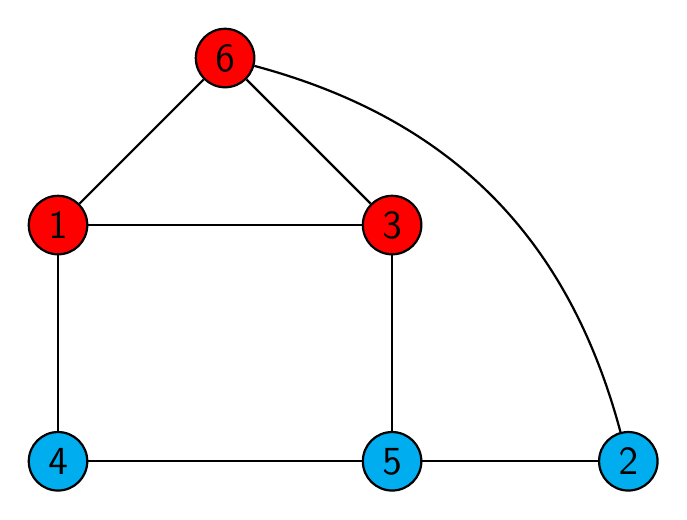
\begin{tikzpicture}[auto, node distance=3cm, every loop/.style={},thick, main node/.style={circle,draw,font=\sffamily\Large}]
            \node[main node, fill=red] (6) {6};
            \node[main node, fill=red] (1) [below left of=6] {1};
            \node[main node, fill=red] (3) [below right of=6] {3};
            \node[main node, fill=cyan] (5) [below of=3] {5};
            \node[main node, fill=cyan] (2) [right of=5] {2};
            \node[main node, fill=cyan] (4) [below of=1] {4};

            \path[every node/.style={font=\sffamily\small}]
                (1) edge (3)
                    edge (4)
                    edge (6)
                (2) edge (5)
                    edge [bend right] (6)
                (3) edge (5)
                    edge (6)
                (4) edge (5);
        \end{tikzpicture}
    \end{figure}
    \FloatBarrier
    \noindent    
    we have
    \[
        \begin{aligned}
            E(S,\overline{S}) &= \set{(1,4),(3,5), (2,6)}\\
            \vol \textcolor{cyan}{S} &= 7\\
            \vol \textcolor{red}{\overline{S}} &= 9
        \end{aligned}
    \]
    So
    \[
        \Phi(\textcolor{cyan}{S}) = \frac{3}{7}
    \]
\end{example}

Looking for the conductance of a graph has also crucial real-world applications. Indeed, it plays a central role in the design of recursive algorithms, image segmentation, community detection, clustering and percolation. For instance, the permeability of petroleum through porous rock can be modelled in terms of the conductance of a graph, with weights given by pore sizes.

\begin{definition}[Graph conductance]
    The conductance of a graph is min conductance of a non trivial cut.
    \[
        \Phi(G) \defeq \min\limits_{\emptyset \neq S \subsetneq V} \Phi(S)
    \]
\end{definition}

\begin{theorem}
    Find the cut minimizing the conductance is \NP-hard.
\end{theorem}

Indeed, the index of $\min$ is over an exponential set ($\mathcal{P}(V)$) $\Ra$ combinatorial explosion of cuts in discrete setting.

We can prove the theorem by reduction from the MAX-CUT problem in cubic graphs which is known to be \NP-Complete~\cite{yannakakis1978node}.

We can notice that the decision problem associated to this optimization problem is "Given $G=(V,E)$ and $\varphi$, is there a non trivial cut $S$ such that $\Phi(S) \leqslant \varphi$?". This problem is obviously \NP. Indeed, is the answer is yes, a sufficient certificate is a cut which achieve the inequality. This certificate is polynomial and can be checked in polytime. Thus, the problem of graph conductance is \NP-complete.

\bigskip

We are going to embed $G$ into $\RR$. We will find some mapping with fine property from $G$ to the real line. We chose $\RR$ because we can hope that the approximation algorithm will work by run through $\RR$ a constant number of times.

We will now define an other quantity related to $\Phi(S)$ but usually easier to manipulate.

\begin{definition}
    \[
        h(S) \defeq \frac{\card{E(S,\overline{S})}}{(\vol S)(\vol \overline{S})} \vol G
    \]
\end{definition}

As we have noticed above
\[
    \vol G = \vol V = \sum\limits_{v\in V} d_v = 2m
\]

Moreover volume is linear for disjoints sets:
\[
    \vol S + \vol \overline{S} = \vol G
\]
We can deduce such properties by considering volume as cardinal of multisets.

Assuming $\vol S \leqslant \vol \overline{S}$,
\[
    \frac{1}{2} \leqslant \frac{\vol \overline{S}}{\vol G} \leqslant 1
\]

We define the h-value as follow :

\begin{definition}
    \[
        \begin{aligned}
            h(G) &\defeq \min\limits_{\emptyset \neq S \subsetneq V} h(S)\\
            &=\min\limits_S \frac{\card{E(S,\overline{S})}}{(\vol S)(\vol \overline{S})} \vol G
        \end{aligned}
    \]
\end{definition}

\[
    \forall S, \Phi(S) \leqslant h(S) \leqslant 2 \Phi(S)
\]
In particular,
\[
    \Phi(G) \leqslant h(G) \leqslant 2 \Phi(G)
\]

We just proved that the h-value is a 2-approximation of the conductance. But the problem remains \NP-hard.

\bigskip

We will now show that this problem in terms of graph can be expressed in terms of functions $\textbf{x} \in \{0,\,1\}^{n}$, easier to manipulate.

So, let us define some probability measures on vertices and cuts as vectors :

\[
    \begin{aligned}
        \nu : E &\to [0,1] \\
           e &\mapsto \frac{1}{m}
    \end{aligned}
\]

$\nu$ is the uniform probability measure defined on the set of edges $E$.

\[
    \begin{aligned}
        \mu : V&\to [0,1]\\
        i &\mapsto \frac{d_i}{2m}
    \end{aligned}
\]

$\mu$ is the probability measure defined on the set of vertices $V$ induced by the degrees.

Then, we can extend these definitions to the subsets $F \subseteq E$ and $S \subseteq V$:

\[
    F\subseteq E,\, \nu(F) = \sum\limits_{e\in F} \nu(e)
\]

\[
    S\subseteq V,\, \mu(S) = \sum\limits_{i\in S} \mu(i)
\]

\begin{notation}
    $1_S \in \RR^V$, the indicator function of $S$:
    \[
        \begin{aligned}
            1_S: S &\to \set{0,1}\\
            i &\mapsto [i\in S]\footnotemark
            = \begin{cases}
                    0 & i\not\in S\\
                    1 & i\in S
                \end{cases}     
        \end{aligned}
    \]
\end{notation}
\footnotetext{\url{https://en.wikipedia.org/wiki/Iverson_bracket}}

We can express $\card{E(S,\overline{S})}$ as
\[
    \card{E(S,\overline{S})} = \sum\limits_{ij\in E} \lvert 1_S(i)-1_S(j)\rvert = \sum\limits_{ij\in E} \left( 1_S(i)-1_S(j)\right)^2 = m \EE_{ij \leftarrow \nu} \left[ \left( 1_S(i)-1_S(j)\right)^2 \right]
\]
indeed, we can partition $E$ in 3 sets: $\set{ij \vert i\in S \wedge j \in S}$ (edges in the graph induced by $S$), $\set{ij \vert i\not\in S \wedge j \not\in S}$ (edges in the graph induced by $\overline{S}$) and $\set{ij \vert i\in S \oplus j \in S}$. For the two firsts, $1_S(i) = 1_S(j)$. But for the last one, $\lvert 1_S(i) - 1_S(j)\rvert = 1$. Moreover, this set is exactly $E(S,\overline{S})$, hence the formula.

We can then express the volume of $S$ as follow:
\[
    \frac{\opname{vol} S}{\opname{vol} G} = \EE_{i \leftarrow \mu} \left[  1_S(i)\right]
\]
because
\[
    \EE_{i \leftarrow \mu} \left[  1_S(i)\right] = \sum_{i\in V} \frac {d_i} {2m} 1_S(i) = \frac { \sum_{i\in S} d_i} {2m} = \frac {\vol S} {\vol G}
\]

We notice that
\[
    \begin{aligned}
        \frac{\vol S}{\vol G} &= \frac{\sum\limits_{i\in S} d_i}{\sum\limits_{i\in G} d_i}\\
        &= \sum\limits_{i\in S}\frac{d_i}{2m}\\
        &= \esp[i\la\mu]{1_S(i)}
    \end{aligned}
\]

Moreover
\[
    \esp[ij\la\nu]{(1_S(i)-1_S(j))^2}
\]
is the fraction of edges which go through the cut, that we can write as
\[
    \frac{\card{E(S,\overline{S})}}{m}
\]


\begin{proposition}
    \[
        h(S) = \frac{\esp[ij\la \nu]{(1_S(i)-1_S(j))^2}}{\esp[(i,j)\la\mu\times\mu]{(1_S(i)-1_S(j))^2}}
    \]
\end{proposition}
\begin{proof}
    In the one hand, we compute the numerator:
    \[
        \begin{aligned}
            \esp[ij\la\nu]{(1_S(i)-1_S(j))^2} &= \frac{\card{E(S,\overline{S})}}{m}\\
            &= \frac{2\card{E(S,\overline{S})}}{\vol G}
        \end{aligned}
    \]
    
    In the other hand, the denominator:
    \[
        \begin{aligned}
            \esp[(i,j)\la\mu\times\mu]{(1_S(i)-1_S(j))^2} &= \esp[(i,j)\la\mu\times\mu]{(1_S(i)+1_S(j)-2\cdot 1_S(i)1_S(j))}\\
            &= 2 \frac{\vol S}{\vol G} -2\esp[(i,j)\la\mu\times\mu]{1_S(i)1_S(j)}\\
            &=2\frac{\vol S}{\vol G} - 2 \left( \frac{\vol S}{\vol G}\right)^2\\
            &\text{\qquad\qquad since }i\text{ and }j\text{ are drawn independently}\\
            &= 2 \frac{\vol S}{\vol G}\left( 1- \frac{\vol S}{\vol G}\right)\\
            &= \frac{2 \vol S \vol \overline{S}}{\vol G \vol G}
        \end{aligned}
    \]
    
    Hence, the ratio is
    \[
        \begin{aligned}
            \frac{\frac{2\card{E(S,\overline{S})}}{\vol G}}{\frac{2 \vol S \vol \overline{S}}{\vol G \vol G}} &= \frac{2\card{E(S,\overline{S})}}{\frac{2 \vol S \vol \overline{S}}{\vol G}}\\
            &= \frac{2\card{E(S,\overline{S})}}{2 \vol S \vol \overline{S}}\vol G\\
            &= h(S)
        \end{aligned}
    \]
\end{proof}

\begin{proposition}
    \[
        \begin{aligned}
            h(G) &= \min\limits_{S} \frac{\overbrace{\esp[ij\la \nu]{(1_S(i)-1_S(j))^2}}^{\text{laplacian of the graph}}}{\underbrace{\esp[(i,j)\la\mu\times\mu]{(1_S(i)-1_S(j))^2}}_{\text{laplacian of the complete graph}}}\\
            &=\min\limits_{x\in\set{0,1}^n} \frac{\esp[ij\la\nu]{(x_i-x_j)^2}}{\esp[(i,j)\la\mu\times\mu]{(x_i-x_j)^2}}\\
            &\geqslant \min\limits_{x\in\RR^n} \frac{\esp[ij\la\nu]{(x_i-x_j)^{2}}}{\esp[(i,j)\la\mu\times\mu]{(x_i-x_j)^2}}
        \end{aligned}
    \]
    The last expression is the relaxation of the problem of the $h$-value of $G$.
\end{proposition}

$x_i$ replaces $1_S(i)$, so the relaxation is about $[i\in S]$. We keep a square in the relaxation instead of absolute value. So, we have a quadratic form and it will be useful to embed $G$ in $\RR$ instead of $\RR^n$.

\[
    \begin{aligned}
        \esp[ij\la\nu]{(x_i-x_j)^2} &= \frac{1}{m} \sum\limits_{ij\in E} (x_i-x_j)^2\\
        &= \frac{1}{m} x^T L x
    \end{aligned}
\]

\[
    \begin{aligned}
        \esp[(i,j) \la \mu\times\mu]{(x_i-x_j)^2} &= \esp[(i,j)\la\mu\times\mu]{{x_i}^2+{x_j}^2-2x_ix_j}\\
        &= 2\esp[i\la \mu]{{x_i}^2} - 2\left( \esp[i\la \mu]{x_i}\right)^2\\
        &= \frac{2}{\vol G} x^T D x\\
        &= \frac{1}{m} x^T D x
    \end{aligned}
\]

So, the relaxation can be rewrite

\[
    \min\limits_{x\in\RR^n} \frac{\esp[ij\la\nu]{(x_i-x_j)^{2}}}{\esp[(i,j)\la\mu\times\mu]{(x_i-x_j)^2}} = \min\limits_{\substack{x\in\RR^n\\\angle{x,D1}=0}} \frac{x^TLx}{x^TDx}
\]


This expression is close to a mathematical program finding an eigen value at the exception of the $D$ in the denominator. To reduce this problem to finding the second smallest eigen value, we can apply the following change of variable: $y = D^{\frac{1}{2}} x$ where 
\[
    D^{\frac{1}{2}} = \left(\begin{matrix}
         \ddots&&0 \\
         & \sqrt{d_i}\\
         0&&\ddots
    \end{matrix}\right)
\]

since $\forall i, d_i >0$.

\[
    \begin{aligned}
        &\min\limits_{\substack{y\in\RR^n\\\angle{D^{- \frac{1}{2}}y,D1}=0}} \frac{(D^{-\frac{1}{2}} y)^T L (D^{-\frac{1}{2}}y)}{y^Ty} &= \min\limits_{\angle{y, D^{\frac{1}{2}}1}=0} \frac{y^T(D^{-\frac{1}{2}}LD^{-\frac{1}{2}})y}{y^T y}
        &= \lambda_2 (\L)
    \end{aligned}
\]
where $\L = D^{-\frac{1}{2}} L D^{-\frac{1}{2}}$ is the normalized Laplacian. We also note that since $D^{\frac{1}{2}}1$ is an eigenvector associated to the smallest eigenvalue of $\L$, we have $\L D^{\frac{1}{2}} 1 =0$.

\[
    \boxed{\L_{i,j} = \frac{L_{i,j}}{\sqrt{d_id_j}}}
\]

\[
    \lambda_2(\L) = h_\RR(G) \leqslant h(G) \leqslant 2\Phi(G)
\]

We have just prove a lower bound on conductance: $\lambda_2(\L) \leqslant 2\Phi(G)$. 

Now we reduced our problem to finding an eigenvalue, this approximation is computable in polynomial time as we have seen previously and then computing the bound is feasible.

Now, we will prove an upper bound of the conductance, the \textsc{Cheeger}'s inequality: $\Phi(G) \leqslant 2\sqrt{\lambda_2(\L)}$. This inequality is convenient since it involve the same eigenvalue.

\paragraph{Part 1}

Reformulate $\Phi(G)$ in term of embeddings.

% Droite réelle avec des y_i dans l'ordre. 
\wtf{}

$\lvert y_i -y_j \rvert \neq (y_i-y_j)^2$. We use square distance.

\[
    \min\limits_{\substack{y\in\RR^n\\\mu_{\frac{1}{2}(y)=0}}} \frac{\esp[ij\la\nu]{\lvert y_i-y_j\rvert}}{\esp[i\la\mu]{\lvert y_i \rvert}} = \Phi(G)
\]

where $\mu_{\frac{1}{2}}$ is the median: any $t$ such that $\mu\set{i\vert y_i < t} \leqslant \frac{1}{2}$ and $\mu\set{i\vert y_i >t} \leqslant \frac{1}{2}$. This value is not well defined. In fact $\mu_{\frac{1}{2}}(i)$ must be a set. But whatever, we will use this notation to designate any element of this set.


\paragraph{Part 2}
\wtf{C'est quoi ce truc ?}
\[
    \frac{\esp[ij\la\nu]{(x_i-x_j)^2}}{\esp[(i,j)\la\mu\times\mu]{(x_i-x_j)^2}} \rightsquigarrow x^*
\]



To prove,
\[
    \min\limits_{\substack{y\in\RR^n\\\mu_{\frac{1}{2}(y)=0}}} \frac{\esp[ij\la\nu]{\lvert y_i-y_j\rvert}}{\esp[i\la\mu]{\lvert y_i \rvert}} = \Phi(G)
\]
we will prove two inequalities ($\leqslant$ and $\geqslant$).

\bigskip

Say $S:=\underset{S}{\argmin}\,\Phi(S)$ ie. the cut achieving the optimal conductance ($\Phi(S) = \Phi(G)$).

\[
    \begin{aligned}
        \frac{\esp[ij\la\nu]{\lvert1_S(i)-1_S(j)\rvert}}{\esp[i\la\mu]{\lvert 1_S(i)\rvert}} &= \frac{\frac{1}{m}\lvert E(S,\overline{S})\rvert}{\frac{\vol S}{2m}}\\
        &= \frac{2\lvert E(S,\overline{S}) \rvert}{\min\set{\vol S, \vol \overline{S}}}\\
        &= 2 \Phi(G)
    \end{aligned}
\]

\bigskip

To prove the other inequality, let's take $y_1 < \cdots < y_n$ be an embedding of $G$ which $\frac{\esp{\lvert y_i-y_j\rvert}}{2\esp{\lvert y_i \rvert}}$. We assume that $\forall (i,j), i\neq j \Ra y_i \neq y_j$.

$\mu_{\frac{1}{2}}(y) = 0$.

% Blabla que je comprends pas pour en arrievr à Chasles.

\begin{notation}
    $S_i = \brackets{1,i}$ and $\overline{S_i} = \brackets{i+1,n}$
\end{notation}

$S_1, S_2,\ldots, S_{n-1}$ "sweep cuts".

\paragraph{Numerator:}

\[
    \sum\limits_{e=ij} \lvert y_i-y_j \rvert = \sum\limits_{i=1}^{n-1} (y_{i+1} - y_i) \lvert E(S_i, \overline{S_i} \rvert
\]

So we have written things in this way\dots.

\paragraph{Denominator:}


\[
    \sum\limits_{i=1}^n \overset{?}{=} \sum\limits_{i=1}^{n-1} (y_{i+1} - y_i) \min(\vol S_i, \vol \overline{S_i})
\]

\[
    \frac{\sum\limits_i \alpha_i n_i}{\sum\limits_i \alpha_i d_i} \geqslant \min\limits_i \frac{n_i}{d_i}
\]

because $\frac{a_1+a_2}{b_1+b_2} \geqslant \min\set{\frac{a_1}{b_1},\frac{a_2}{b_2}}$ which is true if $b_i > 0$.


$\hat{S}$ denotes the cut with min $\Phi$ among $(S_i)_{i\in\brackets{1,n-1}}$.


\[
    \begin{aligned}
        \frac{\sum\limits_i \alpha_i n_i}{\sum\limits_i \alpha_i d_i} \geqslant \min\limits_i \frac{n_i}{d_i} = \min_i \frac{\card{E(S_i,\overline{S_i})}}{\min\set{\vol S_i,\vol \overline{S_i}}} &= \Phi(\hat{S})\\
        &\geqslant \Phi(G)
    \end{aligned}
\]

So, it remains 
\[
    \sum\limits_{i=1}^n \overset{?}{=} \sum\limits_{i=1}^{n-1} (y_{i+1} - y_i) \min(\vol S_i, \vol \overline{S_i})
\]
to prove.


% Encore la droite réelle des y_i. Avec 0 en y_k.

We make the assumption that $\exists k : y_k = 0$. This is just a simplification. We keep the name $k$ for this index.

\[
    \begin{aligned}
        \sum\limits_i d_i\lvert y_i \rvert &= \sum\limits_{i\leqslant k} d_i(-y_i) + \sum\limits_{i > k}d_i y_i\\
       d_i &= \vol S_i - \vol S_{i-1}\\
       \sum\limits_i d_i\lvert y_i \rvert &= \sum\limits_{i\leqslant k} (\vol S_i - \vol S_{i-1})(-y_i) + \sum\limits_{i>k} \left(\vol \overline{S_i} \vol \overline{S_{i+1}} \right)y_i\\
       % On groupe différemment les termes. C'est pas un truc comme Abel ?
       &= \sum\limits_{i\leqslant k} \vol S_i (y_{i+1} -y_i) + \sum\limits_{i>k} \vol \overline{S_i} (y_{i+1} - y_i)
    \end{aligned}
\]

What we have done, to summarize, $\underset{\underset{y(=1_S)}{\downarrow}}{S}$ opt of $\Phi(G)$.

\[
    \min\limits_y \frac{\esp{\lvert y_i-y_j\rvert}}{2\esp{\lvert y_i \rvert}} \leqslant \Phi(G)
\]
Thus, $=$.

Goal $\Phi(G) \leqslant 2\sqrt{\lambda_2(\L)}$. Start with $x$ which obtains $\lambda_2(\L)$.

\[
    \frac{\underset{ij\la \nu}{\EE}(x_i-x_j)^2}{\underset{(i,j)\la\mu\times\mu}{\EE}(x_i-x_j)^2} = \lambda_2(\L)
\]

Produce a $y$ (from $x$) such that
\begin{enumerate}[(1)]
    \item $\mu_{\frac{1}{2}}(y) = 0$
    \item $\frac{\underset{ij\la\nu}{\EE}\lvert y_i-y_j\rvert}{2\underset{i}{\EE}\lvert y_i \rvert} \leqslant (\overset{?}{=}) \sqrt{\lambda_2(\L)}$
\end{enumerate}

$y_i = {x_i}^2 \sgn(x_i)$

\[
    \begin{aligned}
        \underset{ij\la\nu}{\EE} \lvert y_i - y_j \rvert &= \underset{ij \la \nu}{\EE} \lvert \sgn(x_i){x_i}^2 - \sgn(x_j){x_j}^2\rvert\\
        &\leqslant \underset{ij\la \nu}{\EE} \lvert x_i-x_j \rvert(\lvert x_i \rvert + \lvert x_j \rvert)\\
        &\leqslant \sqrt{\underset{ij\la\nu}{\EE}(x_i-x_j)^2} \sqrt{\underset{ij\la \nu}{\EE} (\lvert x_i \rvert + \lvert x_j \rvert)^2}\\
        &\leqslant \sqrt{\underset{ij\la\nu}{\EE}(x_i-x_j)^2} \sqrt{2\underset{ij\la \nu}{\EE} \lvert x_i \rvert^2 + \lvert x_j \rvert^2}\\
        &\leqslant \sqrt{\underset{ij\la\nu}{\EE}(x_i-x_j)^2} \sqrt{4\underset{i\la \mu}{\EE} \lvert y_i \rvert}
    \end{aligned}
\]


So

\[
    \frac{\underset{ij\la\nu}{\EE}\lvert y_i-y_j \rvert}{\underset{i\la\mu}{\EE}\lvert y_i \rvert} \leqslant \sqrt{\frac{4 \underset{ij\la\nu}{\EE}(x_i-x_j)^2}{\underset{i\la\mu}{\EE}\lvert y_i \rvert}} \leqslant\sqrt{8\lambda_2(\L)}
\]

\[
    \Phi(G) \leqslant \sqrt{2\lambda_2(\L)}
\]

\begin{algorithm}[!ht]
    \DontPrintSemicolon
    Compute $x$\;
    $y_i = \sgn(x_i){x_i}^2$\;
    \Return the cut which minimize $\Phi(S_i)$.
\end{algorithm}

\bibliographystyle{alpha}
\bibliography{scribing}

\end{document}
